% MYOPIA -- supplementary material.
% Generated by evaluation/supplementary.py; edit that script, not this file.
%
% Compiles standalone with pdflatex. To drop into the WACV template instead,
% replace the documentclass/geometry lines below with the wacv.sty preamble
% and delete \title/\author/\maketitle.
\documentclass[10pt,twocolumn,letterpaper]{article}
\usepackage[margin=0.75in]{geometry}
\usepackage{booktabs}
\usepackage{graphicx}
\usepackage{amsmath}
\usepackage{amssymb}
\usepackage{times}
\usepackage[hidelinks]{hyperref}
\setcounter{table}{0}
\renewcommand{\thetable}{S\arabic{table}}
\setcounter{figure}{0}
\renewcommand{\thefigure}{S\arabic{figure}}
\setcounter{section}{0}
\renewcommand{\thesection}{S\arabic{section}}

\title{\vspace{-2em}MYOPIA: Understanding the Limits of Tree-Based Reasoning\\
in Vision-Language Models\\[0.4em]\large Supplementary Material}
\author{}
\date{}

\begin{document}
\maketitle
\vspace{-3em}



\section{Scope and Conventions}
\label{sec:supp_scope}

This supplement reports the complete results promised in the Reproducibility
paragraph of the main paper. Section~\ref{sec:supp_full} gives every condition
at both temperatures, including the tree-with-history ablation;
Section~\ref{sec:supp_stats} the paired-bootstrap intervals and corrected
significance tests for the tree--zero-shot gap;
Section~\ref{sec:supp_prompts} the ten-prompt zero-shot sweep;
Section~\ref{sec:supp_repeats} the scope of repeated measurement;
Section~\ref{sec:supp_global} the global-label probe;
Section~\ref{sec:supp_numbered} the numbered-choice probe; and
Sections~\ref{sec:supp_trees}--\ref{sec:supp_audit} the tree specifications,
node counts, and audit coverage. Section~\ref{sec:supp_repro} records the
reproducibility details: the artifacts shipped with this supplement, the fixed
image subsets, the decoding settings, and the limits on exact
re-execution.

Three conventions apply throughout, and are stated here because they determine
how every number below should be read.

\paragraph{Accuracy denominator.} A prediction is correct when the integer
ground-truth class equals the integer predicted class. The denominator is
\emph{every row of the condition}, so an unparseable answer and an image whose
traversal was never logged both count as wrong. Accuracy therefore blends
reasoning failure with answer-interface failure by construction; the two are
separated only in the answer-interface analysis of the main paper and in
Section~\ref{sec:supp_numbered} here.

\paragraph{GTSRB row deduplication.} The GTSRB database contains legacy rows
under \texttt{all\_sequences\_training/} that duplicate images stored under
\texttt{datasets/GTSRB/Training/}. All tables in the main paper and in this
supplement read through a view that drops the legacy copy whenever a matching
modern row exists for the same model, temperature, ablation, and run. Ignoring
this deduplication changes GTSRB denominators from 901 to as many as 915 and
shifts accuracies by up to 0.3 points, so any recomputation that does not
deduplicate will not reproduce these numbers exactly.

\paragraph{Coverage.} A full pass is 901 images for GTSRB, 1000 for MNIST and
CIFAR-10, and 850 for MSCOCO. The main paper prints a cell only when its
condition covers at least 90\% of a full pass. This supplement instead prints
every cell that has data and annotates the incomplete ones with their $n$, so
that what was and was not run to completion is visible rather than hidden.

\section{Complete Results at Both Temperatures}
\label{sec:supp_full}

Table~\ref{tab:supp_full} reports all five prompting conditions at $T{=}0$ and
$T{=}0.7$, extending Table~1 of the main paper with the $T{=}0$ block and the
tree-with-history (Tree+H) ablation.

Two features of the table deserve comment. First, the $T{=}0$ block is complete
only for GTSRB and CIFAR-10. On MNIST and MSCOCO the $T{=}0$ conditions were
not run to completion, and the surviving cells cover between 2 and 860 images;
they are printed with their $n$ but should not be read as dataset-level
estimates. This is the reason the main paper restricts its $T{=}0$ discussion to
GTSRB and CIFAR-10.

Second, Tree+H is a full pass only on GTSRB and CIFAR-10. On MNIST and MSCOCO
it covers 2--33 images, so the apparently strong values there (for example
75.00 for GPT-4o on MNIST, from 16 images) carry no weight. The
history ablation should be read from the GTSRB and CIFAR-10 rows alone, where
it reduces accuracy in five of six comparisons, the single exception being
Qwen-VL on GTSRB.

Best and second-best marking considers only cells at full coverage, so a
partial cell can never be marked as a winner.


\begin{table*}[t]
\centering
\caption{Complete accuracy (\%) for every condition at both temperatures. ZS: zero-shot; +D: class and image descriptions injected into the prompt; +H: conversation history carried across tree nodes; CoT: chain-of-thought. Accuracy counts unparseable answers and images with no logged traversal as wrong, so every cell shares the denominator of its condition. Superscripts give $n$ for cells that did not complete a full dataset pass ($<90\%$ coverage); an em dash marks conditions with no logged rows. CoT was run at $T{=}0.7$ only, on a $n{=}100$ probe per dataset--model pair with full class coverage. Bold and underlined values denote the best and second-best result within each dataset--model--temperature row, considering only cells at full coverage. Full passes are $n=901$ (GTSRB), $1000$ (MNIST, CIFAR-10), and $850$ (MSCOCO).}
\label{tab:supp_full}
\footnotesize
\setlength{\tabcolsep}{4.6pt}
\begin{tabular}{@{}ll c rrrrrr@{}}
\toprule
\textbf{Dataset} & \textbf{Model} & $T$ & \textbf{ZS} & \textbf{ZS+D} & \textbf{CoT} & \textbf{Tree} & \textbf{Tree+H} & \textbf{Tree+D} \\
\midrule
GTSRB     & GPT-4o   & $0$ &   \textbf{70.92} &            63.82 &              --- &            58.05 &            55.83 & \underline{66.81} \\
          &          & $0.7$ &   \textbf{71.14} &            63.60 &            63.00 &            57.71 &            56.71 & \underline{65.04} \\
\cmidrule(l){2-9}
          & LLaMA    & $0$ &   \textbf{23.86} & \underline{18.42} &              --- &             6.33 &            16.09 &            15.65 \\
          &          & $0.7$ &   \textbf{37.07} &            23.53 &            12.00 & \underline{33.19} &            12.43 &            14.87 \\
\cmidrule(l){2-9}
          & Qwen-VL  & $0$ &            47.95 & \underline{49.72} &              --- &            40.51 &            36.96 &   \textbf{51.83} \\
          &          & $0.7$ &            47.06 & \underline{48.95} &            36.00 &            24.64 &            36.96 &   \textbf{52.28} \\
\midrule
MNIST     & GPT-4o   & $0$ &  94.87$^{\,234}$ &  88.02$^{\,860}$ &              --- &  35.47$^{\,234}$ &   46.67$^{\,15}$ &              --- \\
          &          & $0.7$ & \underline{91.50} &            86.40 &   \textbf{94.00} &            34.60 &   75.00$^{\,16}$ &            28.60 \\
\cmidrule(l){2-9}
          & LLaMA    & $0$ &    33.33$^{\,3}$ &              --- &              --- &    33.33$^{\,3}$ &     0.00$^{\,2}$ &              --- \\
          &          & $0.7$ & \underline{59.30} &            40.20 &   \textbf{71.00} &             7.70 &    50.00$^{\,2}$ &             2.60 \\
\cmidrule(l){2-9}
          & Qwen-VL  & $0$ &  95.17$^{\,414}$ &              --- &              --- &  14.25$^{\,414}$ &              --- &              --- \\
          &          & $0.7$ &   \textbf{94.40} & \underline{89.20} &            86.00 &            29.30 &    7.69$^{\,13}$ &            27.10 \\
\midrule
CIFAR-10  & GPT-4o   & $0$ & \underline{89.60} &   \textbf{90.00} &              --- &            75.40 &            73.10 &            82.70 \\
          &          & $0.7$ & \underline{87.90} &   \textbf{88.90} &            87.00 &            76.00 &            72.80 &            80.60 \\
\cmidrule(l){2-9}
          & LLaMA    & $0$ & \underline{43.70} &   \textbf{62.80} &              --- &            17.10 &            12.30 &             4.80 \\
          &          & $0.7$ &            36.70 &   \textbf{54.00} & \underline{38.00} &            16.40 &            14.10 &             6.00 \\
\cmidrule(l){2-9}
          & Qwen-VL  & $0$ &   \textbf{77.60} & \underline{71.20} &              --- &            56.60 &            33.00 &            66.50 \\
          &          & $0.7$ &   \textbf{77.60} & \underline{70.90} &            63.00 &            56.60 &            33.00 &            66.30 \\
\midrule
MSCOCO    & GPT-4o   & $0$ &   73.91$^{\,92}$ &              --- &              --- &   46.74$^{\,92}$ &     0.00$^{\,7}$ &              --- \\
          &          & $0.7$ & \underline{72.82} &   \textbf{80.82} &            71.00 &            46.71 &   33.33$^{\,33}$ &            44.00 \\
\cmidrule(l){2-9}
          & LLaMA    & $0$ &    50.00$^{\,2}$ &              --- &              --- &     0.00$^{\,2}$ &     0.00$^{\,4}$ &              --- \\
          &          & $0.7$ &   \textbf{23.76} & \underline{21.06} &            18.00 &             3.65 &    33.33$^{\,6}$ &             0.35 \\
\cmidrule(l){2-9}
          & Qwen-VL  & $0$ &  76.47$^{\,221}$ &              --- &              --- &  40.27$^{\,221}$ &              --- &              --- \\
          &          & $0.7$ & \underline{74.82} &   \textbf{78.35} &            59.00 &            39.65 &              --- &            44.47 \\
\bottomrule
\end{tabular}
\end{table*}


\section{Significance of the Tree--Zero-Shot Gap}
\label{sec:supp_stats}

Table~\ref{tab:supp_full} shows the tree condition below zero-shot almost
everywhere. Table~\ref{tab:supp_bootstrap} attaches an interval and a
corrected $p$-value to that gap, so the claim rests on more than a point
estimate.

The design is paired: for a given dataset, model, and temperature, the
zero-shot and tree predictions for one image are stored on the same database
row, so the two conditions see identical images. The bootstrap therefore
resamples \emph{images}, not predictions, and recomputes both accuracies on
each resample; the reported interval is over the difference, which absorbs the
correlation between the two conditions rather than treating them as
independent samples.

Two limits are worth stating. The two-sided bootstrap $p$ cannot fall below
$2/10{,}000$, so eleven of the twelve comparisons report that floor and the
corrected values for them are upper bounds rather than exact
quantities. And the interval covers sampling variation over images at a fixed
decoding temperature; it does not cover run-to-run decoding variation, which is
the separate quantity measured in Section~\ref{sec:supp_repeats}.

All twelve gaps are negative, and all twelve remain significant after
Holm--Bonferroni correction over the family of twelve comparisons (largest
adjusted $p=0.0278$, GTSRB with LLaMA). The single smallest gap,
$-3.88$ points for LLaMA on GTSRB, is also the only one whose interval
approaches zero ($[-7.33, -0.44]$); every other interval excludes zero by a
wide margin.


\begin{table*}[t]
\centering
\caption{Paired bootstrap over images for the tree-minus-zero-shot accuracy gap at $T{=}0.7$ (no descriptions, no history, run~0). Zero-shot and tree predictions share an image row, so images are resampled with replacement ($10{,}000$ resamples, seed~42) and both accuracies are recomputed on each resample. $\Delta$ is Tree$-$ZS in points; the interval is the $2.5$--$97.5$ percentile range of the resampled $\Delta$. $p_{\text{Holm}}$ is the two-sided bootstrap $p$ after Holm--Bonferroni correction over all twelve dataset--model comparisons. Entries marked $<$ are floored by bootstrap resolution and are upper bounds. Every comparison is negative and every corrected $p$ clears $\alpha=0.05$.}
\label{tab:supp_bootstrap}
\footnotesize
\setlength{\tabcolsep}{5pt}
\begin{tabular}{@{}llrrrrcr@{}}
\toprule
\textbf{Dataset} & \textbf{Model} & $n$ & \textbf{ZS} & \textbf{Tree} & $\Delta$ & \textbf{95\% CI} & $p_{\text{Holm}}$ \\
\midrule
GTSRB & GPT-4o & 901 & 71.14 & 57.71 & $-13.43$ & $[-16.43, -10.54]$ & $<$0.0024 \\
GTSRB & LLaMA & 901 & 37.07 & 33.19 & $-3.88$ & $[-7.33, -0.44]$ & 0.0278 \\
GTSRB & Qwen-VL & 901 & 47.06 & 24.64 & $-22.42$ & $[-25.64, -19.20]$ & $<$0.0024 \\
\midrule
MNIST & GPT-4o & 1000 & 91.50 & 34.60 & $-56.90$ & $[-60.00, -53.70]$ & $<$0.0024 \\
MNIST & LLaMA & 1000 & 59.30 & 7.70 & $-51.60$ & $[-55.00, -48.10]$ & $<$0.0024 \\
MNIST & Qwen-VL & 1000 & 94.40 & 29.30 & $-65.10$ & $[-68.10, -62.10]$ & $<$0.0024 \\
\midrule
CIFAR-10 & GPT-4o & 1000 & 87.90 & 76.00 & $-11.90$ & $[-14.50, -9.40]$ & $<$0.0024 \\
CIFAR-10 & LLaMA & 1000 & 36.70 & 16.40 & $-20.30$ & $[-23.80, -16.80]$ & $<$0.0024 \\
CIFAR-10 & Qwen-VL & 1000 & 77.60 & 56.60 & $-21.00$ & $[-24.10, -17.90]$ & $<$0.0024 \\
\midrule
MSCOCO & GPT-4o & 850 & 72.82 & 46.71 & $-26.12$ & $[-29.88, -22.47]$ & $<$0.0024 \\
MSCOCO & LLaMA & 850 & 23.76 & 3.65 & $-20.12$ & $[-23.06, -17.18]$ & $<$0.0024 \\
MSCOCO & Qwen-VL & 850 & 74.82 & 39.65 & $-35.18$ & $[-38.82, -31.41]$ & $<$0.0024 \\
\bottomrule
\end{tabular}
\end{table*}


\section{Ten-Prompt Zero-Shot Sweep}
\label{sec:supp_prompts}

The main paper notes that VLMs are sensitive to prompt phrasing and reports
zero-shot results from one prompt. This section gives the full sweep behind
that choice. Ten paraphrases of the zero-shot instruction were written per
dataset; they differ in register and verbosity but request the same output, a
single class ID. The prompt index is stored as \texttt{RunId}, and prompt~0 is
the one reported in Table~1 of the main paper.

Table~\ref{tab:supp_prompt_sweep} and Figure~\ref{fig:supp_prompt_sweep} give
per-prompt accuracy for the six dataset--model pairs where all ten prompts were
run at full scale. Two observations follow, and both qualify the main paper's
zero-shot numbers.

\paragraph{Prompt sensitivity is large, not small.} Across-prompt standard
deviations range from 2.81 points (CIFAR-10, GPT-4o) to 16.97 points (GTSRB,
Qwen-VL), and the max--min spread reaches 41.5 points on GTSRB for Qwen-VL and
31.1 points for LLaMA. Prompt choice is therefore a first-order factor in the
zero-shot number, comparable in magnitude to the differences between models.
The spread is driven partly by catastrophic prompts: Qwen-VL falls to 5.55\% on
one GTSRB paraphrase and 50.1\% on one CIFAR-10 paraphrase, patterns consistent
with format non-compliance rather than a graded loss of recognition ability.

\paragraph{Prompt~0 is the strongest GTSRB prompt, not a typical one.} On
GTSRB, prompt~0 gives the highest accuracy of all sweep prompts for all three
models: 71.14 against a mean of 59.67 for GPT-4o, 37.07 against 16.57 for
LLaMA, and 47.06 against 35.84 for Qwen-VL. On CIFAR-10 it is close to the mean
for GPT-4o (87.90 against 87.08) but above it for Qwen-VL (77.60 against 71.01)
and below it for LLaMA (36.70 against 42.13). The GTSRB zero-shot column of
Table~1 is thus a best-prompt figure rather than a typical-prompt figure.

This matters for the central Tree--zero-shot comparison, because tree traversal
was run only under prompt~0 (Section~\ref{sec:supp_repeats}) and the tree
prompt does not vary with the prompt index. The comparison therefore places a
best-case zero-shot configuration against a single tree configuration on GTSRB.
We report this explicitly rather than reselecting a prompt: the direction of
the gap is unchanged, since even the weakest GTSRB zero-shot prompt for GPT-4o
(45.84) is within 12 points of the tree result and the mean across prompts
(59.67) still exceeds it, but the magnitude of the GTSRB gap should be read as
an upper bound.


\begin{table*}[t]
\centering
\caption{Zero-shot accuracy (\%) for each of the ten prompt paraphrases at $T{=}0.7$, on the datasets where every prompt was run at full scale. P0 is the prompt reported in Table~1 of the main paper. Empty cells are prompts whose run did not reach full coverage and are excluded from the summary statistics. $\Delta$ is $\max-\min$ across prompts.}
\label{tab:supp_prompt_sweep}
\footnotesize
\setlength{\tabcolsep}{4pt}
\begin{tabular}{@{}llrrrrrrrrrr@{\hspace{6pt}}rrr@{}}
\toprule
\textbf{Dataset} & \textbf{Model} & \textbf{P0} & \textbf{P1} & \textbf{P2} & \textbf{P3} & \textbf{P4} & \textbf{P5} & \textbf{P6} & \textbf{P7} & \textbf{P8} & \textbf{P9} & \textbf{Mean} & \textbf{SD} & $\boldsymbol{\Delta}$ \\
\midrule
GTSRB     & GPT-4o   & \underline{71.14} &            63.71 &              --- &            66.04 &            45.84 &            56.16 &            67.70 &            49.94 &              --- &            56.83 & 59.67 & 8.94 & 25.31 \\
          & LLaMA    & \underline{37.07} &            23.20 &            15.54 &            20.75 &            11.10 &            17.09 &            18.87 &             8.10 &             5.99 &             7.99 & 16.57 & 9.28 & 31.08 \\
          & Qwen-VL  & \underline{47.06} &            46.95 &            46.06 &            45.84 &             5.55 &            45.84 &            46.06 &            11.88 &            17.31 &            45.84 & 35.84 & 16.97 & 41.51 \\
\midrule
CIFAR-10  & GPT-4o   & \underline{87.90} &            86.20 &            88.70 &            86.50 &            89.70 &            89.50 &            86.70 &            87.20 &            79.90 &            88.50 & 87.08 & 2.81 & 9.80 \\
          & LLaMA    & \underline{36.70} &            51.00 &            43.10 &            36.10 &            41.20 &            41.60 &            40.90 &            45.10 &            40.10 &            45.50 & 42.13 & 4.38 & 14.90 \\
          & Qwen-VL  & \underline{77.60} &            78.40 &            76.50 &            50.10 &            77.70 &            57.00 &            78.50 &            56.90 &            78.60 &            78.80 & 71.01 & 11.45 & 28.70 \\
\bottomrule
\end{tabular}
\end{table*}

\begin{figure}[t]
\centering
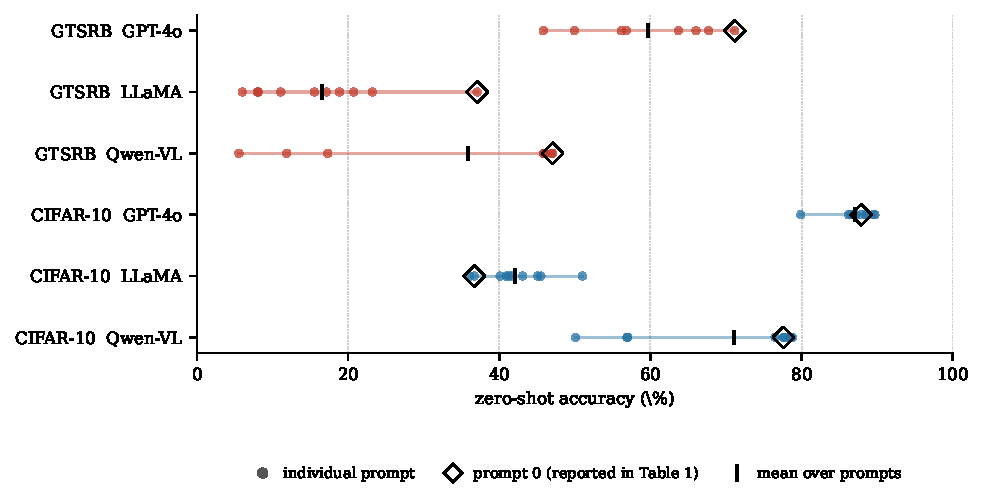
\includegraphics[width=\linewidth]{zs_prompt_sweep.pdf}
\caption{Zero-shot accuracy for each of the ten prompt paraphrases, on the dataset--model pairs swept at full scale. Prompt~0, reported in Table~1 of the main paper, is the best of the ten on GTSRB for all three models.}
\label{fig:supp_prompt_sweep}
\end{figure}


\section{Scope of Repeated Measurement}
\label{sec:supp_repeats}

We state precisely what the repeated-measurement axis in our released databases
does and does not cover, since this bounds the stability claims that can be
made from them.

The \texttt{RunId} field selects the zero-shot prompt paraphrase. All ten
paraphrases are distinct in every dataset. Consequently the variation
quantified in Section~\ref{sec:supp_prompts} is \emph{prompt} variation, and it
applies to the zero-shot condition only.

Tree traversal was executed under \texttt{RunId}~0 alone; the tree prompt is
built from the node's own question and answer set and does not depend on the
prompt index. The database therefore contains one tree traversal per
dataset--model--temperature--ablation cell, and no repeated-run replicate of a
tree result exists at any scale. Reported tree accuracies are single-run
measurements, and we make no claim about their run-to-run stability. Readers
should treat the tree column of every table in the main paper and this
supplement accordingly, and we regard replicated tree runs as the most
important missing robustness check in this release.

Where a full-scale sweep is unavailable, Table~\ref{tab:supp_matched_prompts}
reports the small prompt checks that were run on MNIST and MSCOCO, restricted
to the images all prompts share so the spread reflects prompt choice rather
than differing image subsets. Three of the four checks are stable
(SD $\leq 2.9$ points), but MSCOCO with GPT-4o varies more (SD 4.79 points,
range 65.0--75.0 on 20 images). These checks use 20 images each; their standard
errors are wide and they do not substitute for a full-scale sweep.


\begin{table}[t]
\centering
\caption{Small-scale prompt checks on the datasets without a full-scale sweep. Each row compares the prompts that were run on the same matched image subset, so the spread is not confounded by which images each prompt saw.}
\label{tab:supp_matched_prompts}
\footnotesize
\begin{tabular}{@{}llrrrrr@{}}
\toprule
\textbf{Dataset} & \textbf{Model} & $n$ & \textbf{Prompts} & \textbf{Mean} & \textbf{SD} & $\boldsymbol{\Delta}$ \\
\midrule
MNIST     & GPT-4o   & 20 & 4 & 93.75 & 2.50 & 5.00 \\
          & Qwen-VL  & 20 & 4 & 97.50 & 2.89 & 5.00 \\
MSCOCO    & GPT-4o   & 20 & 4 & 68.75 & 4.79 & 10.00 \\
          & Qwen-VL  & 20 & 4 & 68.75 & 2.50 & 5.00 \\
\bottomrule
\end{tabular}
\end{table}


\section{Global-Label Probe}
\label{sec:supp_global}

Tree traversal shows the model only the current node's answer options, whereas
zero-shot prompting shows it the entire label set. If that difference in label
access were the primary cause of the Tree--zero-shot gap, restoring the global
label list to each node prompt should recover much of it. This probe tests
that, with GPT-4o, on class-stratified subsamples: each node prompt is issued
twice, once in the standard local-list form and once with the dataset's full
class list appended.

Table~\ref{tab:supp_global} reports both conditions on the images the two
conditions share. The global list produces small and inconsistent changes in
node accuracy: $+1.0$ point on GTSRB, $+0.1$ on MSCOCO, $-1.4$ on CIFAR-10 and
$-5.3$ on MNIST. Image-level accuracy moves by $+4$, $+4$, $-5$, and $0$ points
respectively. No dataset approaches its zero-shot accuracy from Table~1. The
global list also slightly \emph{raises} the unresolved rate on three of four
datasets, consistent with the longer prompt making format compliance harder
rather than easier.

We therefore find no support for label access as the primary cause of the gap.
The probe uses 20--50 images per dataset, so it excludes only a large effect;
differences of a few points are not resolvable at this scale.


\begin{table}[t]
\centering
\caption{Global-label probe with GPT-4o, on the images both conditions share. Local is the standard node prompt; Global appends the dataset's full class list to every node prompt. All values are percentages.}
\label{tab:supp_global}
\footnotesize
\setlength{\tabcolsep}{4pt}
\begin{tabular}{@{}lrrrrrrr@{}}
\toprule
& & \multicolumn{2}{c}{\textbf{Node acc.}} & \multicolumn{2}{c}{\textbf{Unresolved}} & \multicolumn{2}{c}{\textbf{Image acc.}} \\
\cmidrule(lr){3-4} \cmidrule(lr){5-6} \cmidrule(l){7-8}
\textbf{Dataset} & $n_{\text{img}}$ & \textbf{Local} & \textbf{Global} & \textbf{Local} & \textbf{Global} & \textbf{Local} & \textbf{Global} \\
\midrule
GTSRB     & 50 & 89.1 & 90.1 & 2.1 & 3.1 & 58.0 & 62.0 \\
MNIST     & 20 & 71.1 & 65.8 & 0.0 & 0.0 & 35.0 & 35.0 \\
CIFAR-10  & 20 & 88.9 & 87.5 & 1.6 & 7.8 & 65.0 & 60.0 \\
MSCOCO    & 50 & 91.2 & 91.3 & 0.3 & 3.8 & 46.0 & 50.0 \\
\bottomrule
\end{tabular}
\end{table}


\section{Numbered-Choice Probe}
\label{sec:supp_numbered}

Because the strict extractor marks a response unresolved whenever it fails to
match a predefined answer, part of the tree deficit could be an
answer-interface artefact rather than a reasoning failure. This probe
prospectively controls for that: on the same images, each node is asked twice,
once with the free-form prompt and strict regex extraction, and once with an
explicit numbered-option format that requests only an option number.

Table~\ref{tab:supp_numbered} reports both conditions. The numbered format
eliminates unresolved responses entirely (0.0\% on all four datasets), while
free-form is already close to fully parseable for GPT-4o (0.0--2.4\%
unresolved). Node accuracy moves by at most a few points and not consistently
in one direction.

\paragraph{A caveat on matching.} Each traversal terminates at its first
incorrect or unresolved decision, so the two conditions do not visit the same
number of nodes even on the same image: a condition that fails earlier
accumulates fewer, shallower, and therefore easier nodes. The node accuracies
in Table~\ref{tab:supp_numbered} are computed over each condition's own node
set, which is what the main paper reports.
Table~\ref{tab:supp_numbered_paired} instead restricts to nodes reached at the
same depth on the same image in both conditions. Matching in this stricter
sense increases the MNIST gain from $+3.1$ to $+8.4$ points and deepens the
MSCOCO loss from $-1.5$ to $-3.8$ points, while GTSRB and CIFAR-10 are
essentially unchanged.

\paragraph{A caveat on power.} The probe uses 20 images per dataset, yielding
36--110 node decisions per condition. None of the four differences is
distinguishable from zero (Fisher exact, all $p > 0.75$), and at the image
level the direction reverses on two datasets. The correct reading is that this
probe excludes a \emph{large} interface effect for GPT-4o, not that it measures
a small one. Notably, free-form unresolved rates here are far below GPT-4o's
rate in the full run (9.9\% on GTSRB), which is what supports the main paper's
claim that GPT-4o's interface failures are concentrated in particular
conditions rather than inherent to free-form prompting.


\begin{table}[t]
\centering
\caption{Numbered-choice probe with GPT-4o ($n{=}20$ images per dataset). Free is the free-form prompt with strict regex extraction; Num.\ requests only an option number. Node accuracy is computed over each condition's own visited nodes, as in the main paper. All values are percentages.}
\label{tab:supp_numbered}
\footnotesize
\setlength{\tabcolsep}{4pt}
\begin{tabular}{@{}lrrrrrrr@{}}
\toprule
& & \multicolumn{2}{c}{\textbf{Node acc.}} & \multicolumn{2}{c}{\textbf{Unresolved}} & \multicolumn{2}{c}{\textbf{Image acc.}} \\
\cmidrule(lr){3-4} \cmidrule(lr){5-6} \cmidrule(l){7-8}
\textbf{Dataset} & $n_{\text{img}}$ & \textbf{Free} & \textbf{Num.} & \textbf{Free} & \textbf{Num.} & \textbf{Free} & \textbf{Num.} \\
\midrule
GTSRB     & 20 & 89.0 & 90.7 & 1.4 & 0.0 & 60.0 & 65.0 \\
MNIST     & 20 & 68.3 & 71.4 & 2.4 & 0.0 & 35.0 & 30.0 \\
CIFAR-10  & 20 & 92.3 & 92.2 & 1.5 & 0.0 & 75.0 & 75.0 \\
MSCOCO    & 20 & 88.2 & 86.7 & 0.0 & 0.0 & 35.0 & 30.0 \\
\bottomrule
\end{tabular}
\end{table}

\begin{table}[t]
\centering
\caption{Numbered-choice probe restricted to nodes reached at the same depth on the same image in both conditions. Matching changes the MNIST and MSCOCO deltas relative to Table~\ref{tab:supp_numbered}.}
\label{tab:supp_numbered_paired}
\footnotesize
\begin{tabular}{@{}lrrrr@{}}
\toprule
\textbf{Dataset} & \textbf{Paired nodes} & \textbf{Free} & \textbf{Num.} & $\boldsymbol{\Delta}$ \\
\midrule
GTSRB     & 73 & 89.0 & 90.4 & +1.4 \\
MNIST     & 36 & 69.4 & 77.8 & +8.3 \\
CIFAR-10  & 63 & 92.1 & 92.1 & +0.0 \\
MSCOCO    & 105 & 90.5 & 86.7 & -3.8 \\
\bottomrule
\end{tabular}
\end{table}


\section{Tree Specifications and Node Counts}
\label{sec:supp_trees}

Table~\ref{tab:supp_tree_specs} gives the structure of the four evaluated
trees. Every internal node has at least two children, every leaf maps to
exactly one class, and no question repeats along any root-to-leaf path.

The trees differ substantially in shape. CIFAR-10 and MNIST are shallow
(maximum depth 3) with 8--9 internal nodes; MSCOCO is an 89-node binary tree of
depth up to 10; and GTSRB is the most irregular, mixing 16 binary nodes with
two ternary, two five-way, and two eight-way nodes, and reaching depth 14. The
eight-way arrow-direction question on GTSRB is the node an independent LLM
judge flagged for question design, and it is also the highest-entropy split in
any of the trees (3.00 bits).

Five MSCOCO internal nodes were never reached by any
primary-condition traversal. They are excluded from the audit because they
have no measured accuracy, which is why the audit covers 123 rather
than 128 nodes.


\begin{table*}[t]
\centering
\caption{Specifications of the four evaluated trees. Branching gives the multiset of child counts over internal nodes. Split entropy $H_v$ is in bits, unnormalised. "Unreached" counts internal nodes that no primary-condition traversal ever visited.}
\label{tab:supp_tree_specs}
\footnotesize
\setlength{\tabcolsep}{4pt}
\begin{tabular}{@{}lrrrlrrr@{}}
\toprule
\textbf{Dataset} & \textbf{Int.} & \textbf{Leaves} & \textbf{Depth} & \textbf{Branching} & $\boldsymbol{\bar{H}}$ & $\boldsymbol{H}$ \textbf{range} & \textbf{Unreached} \\
\midrule
GTSRB     & 22 & 43 & 14 & 16$\times$2, 2$\times$3, 2$\times$5, 2$\times$8 & 1.02 & 0.35--3.00 & 0 \\
MNIST     & 8 & 10 & 3 & 7$\times$2, 1$\times$3 & 1.01 & 0.92--1.30 & 0 \\
CIFAR-10  & 9 & 10 & 3 & 9$\times$2 & 0.96 & 0.81--1.00 & 0 \\
MSCOCO    & 89 & 90 & 10 & 89$\times$2 & 0.93 & 0.54--1.00 & 5 \\
\midrule
\textbf{Total} & \textbf{128} & \textbf{153} & & & & & \textbf{5} \\
\bottomrule
\end{tabular}
\end{table*}


\section{Tree-Quality Audit Coverage}
\label{sec:supp_audit}

Table~\ref{tab:supp_audit_coverage} shows how the 347 node--model
observations of the audit distribute over datasets and models. A node--model
pair enters the audit only when it has both an in-traversal accuracy and a
grounding gap; 1 of the 348 candidate rows lack one of the
two and are dropped.

Coverage is strongly uneven. MSCOCO contributes 237 of the
347 observations (68\%) from 83 nodes, while
MNIST contributes 22 from 7 nodes. Any pooled
association reported in the audit is therefore weighted towards the MSCOCO
tree, which is also the only deep binary tree in the set. This is the main
reason the audit's conclusions are limited to the four evaluated trees and are
not presented as general properties of hierarchical classifiers.

Per-model coverage is 123 nodes for GPT-4o, 121 for Qwen-VL
Max, and 103 for LLaMA-3.2; LLaMA reaches fewer nodes because its
traversals terminate earlier.
Node accuracy in the audit is thus conditional on reach, and nodes deep in a
tree are scored on the subset of traversals that arrived there correctly.


\begin{table}[t]
\centering
\caption{Tree-quality audit coverage. A node--model observation is retained when it has both an in-traversal accuracy and a grounding gap.}
\label{tab:supp_audit_coverage}
\footnotesize
\begin{tabular}{@{}lrr@{}}
\toprule
\textbf{Dataset} & \textbf{Nodes} & \textbf{Node--model pairs} \\
\midrule
GTSRB     & 21 & 61 \\
MNIST     & 7 & 22 \\
CIFAR-10  & 8 & 27 \\
MSCOCO    & 83 & 237 \\
\midrule
\textit{GPT-4o} & & 123 \\
\textit{LLaMA} & & 103 \\
\textit{Qwen-VL} & & 121 \\
\midrule
\textbf{Total} & \textbf{123} & \textbf{347} \\
\bottomrule
\end{tabular}
\end{table}


\section{Reproducibility Details}
\label{sec:supp_repro}

This section records what a reader needs in order to regenerate the numbers
above, and what cannot be regenerated exactly.

\paragraph{Artifacts in this supplement.} The accompanying archive contains the
four evaluated decision trees in full (both the human-readable and the
machine-readable form), the complete prompt set (zero-shot paraphrases,
per-class descriptions, and the node-question templates), the
generator--evaluator tree-construction pipeline, the evaluation harness, and
the analysis scripts that emit every table in this document. It excludes API
credentials, raw provider traces, and the datasets themselves.

\paragraph{Sampling.} Each dataset is evaluated on a fixed image subset, listed
by identifier in the archive: 901 GTSRB, 1000 MNIST, 1000 CIFAR-10, and 850
MSCOCO images. The MSCOCO subset is restricted to images carrying exactly one
category label, so that a single ground-truth class is well defined. These
identifier lists are the sampling record; the subsets are not redrawn at run
time.

\paragraph{Decoding.} All primary conditions use temperature $0$ or $0.7$ with
provider defaults otherwise, one image per request, and no few-shot examples.
Tree traversal issues one request per visited node; the tree-with-history
ablation additionally carries prior node questions and answers forward in the
conversation.

\paragraph{Determinism and its limits.} The analysis layer is deterministic:
the bootstrap fixes seed~42 with $10{,}000$ resamples, and every table is
recomputed from the stored databases rather than from cached summaries. The
generation layer is not. All three models are served through hosted APIs, so
even $T{=}0$ is not bit-reproducible, and the providers may retire or silently
update a checkpoint. The LLaMA endpoint used for the main runs was in fact
retired during the study and replaced by a self-hosted deployment of the same
official weights at fp16. Re-running the pipeline should therefore reproduce
the qualitative ordering and the sign of every gap in
Table~\ref{tab:supp_bootstrap}, but not the exact percentages.

\paragraph{Recomputation path.} The stored databases are the ground truth for
every table here. Given them, the analysis scripts in the archive regenerate
this entire document, including the figure, without any API access or API key.
Reproducing the databases themselves requires API credentials and paid calls.

\paragraph{Known pitfalls.} Two details silently change results if missed. The
GTSRB deduplication described in Section~\ref{sec:supp_scope} must be applied
or GTSRB denominators inflate from 901 to as many as 915. And accuracy counts
unparseable answers and unlogged traversals as wrong; scoring only the
parseable subset raises every tree number and is not comparable to the values
reported here.


\end{document}
